\documentclass[border=15pt, multi, tikz]{standalone}
%\usepackage{blocks}
\usepackage{import}
\subimport{../../layers/}{init}
\usetikzlibrary{positioning}
\usetikzlibrary{3d}

\def\ConvColor{rgb:yellow,5;red,2.5;white,5}
\def\ConvReluColor{rgb:yellow,5;red,5;white,5}
\def\RecColor{rgb:blue,5;green,2.5;white,5}
\def\PoolColor{rgb:red,1;black,0.3}
\def\FcColor{rgb:blue,5;red,2.5;white,5}
\def\FcReluColor{rgb:blue,5;red,5;white,4}
\def\SoftmaxColor{rgb:magenta,5;black,7}

\begin{document}
\begin{tikzpicture}
\Large
\tikzstyle{connection}=[ultra thick,every node/.style={sloped,allow upside down},draw=\edgecolor,opacity=0.7]
%%%%%%%%%%%%%%%%%%%%%%%%%%%%%%%%%%%%%%%%%%%%%%%%%%%%%%%%%%%%%%%%%%%%%%%%%%%%%%%%%%%%%%%%
%% Draw Layer Blocks
%%%%%%%%%%%%%%%%%%%%%%%%%%%%%%%%%%%%%%%%%%%%%%%%%%%%%%%%%%%%%%%%%%%%%%%%%%%%%%%%%%%%%%%%
\node[canvas is zy plane at x=0] (temp) at (-2,0,-4) {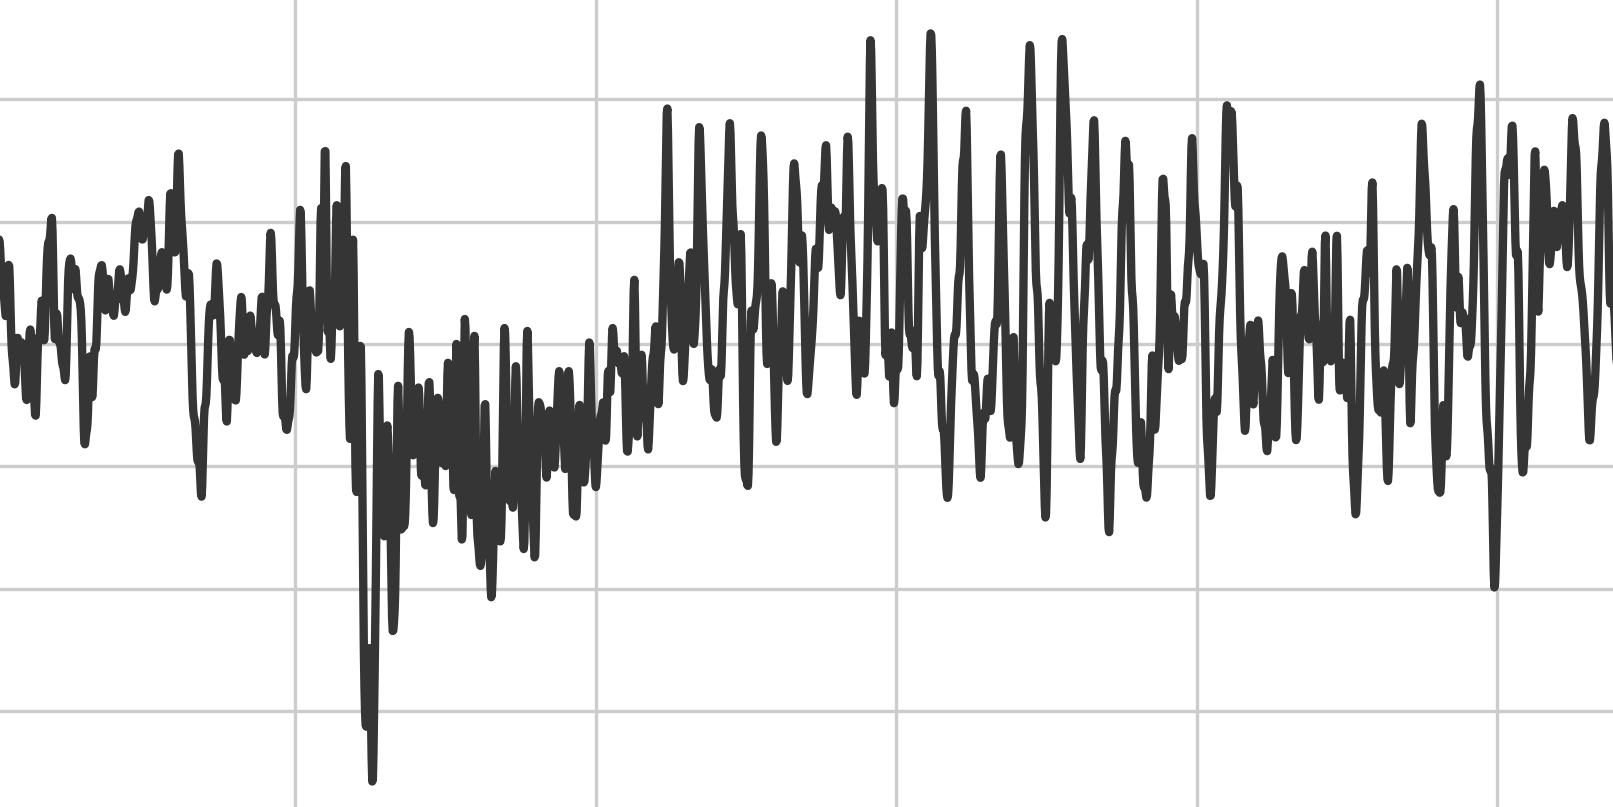
\includegraphics[width=12cm,height=4cm]{signal.png}};

% conv1_1,conv1_2
\pic[shift={(0,0,0)}] at (0,0,0) {RightBandedBox={name=cr1,caption=conv1,%
		xlabel={{"128",}},zlabel=798,fill=\ConvColor,bandfill=\ConvReluColor,%
		height=5,width=8,depth=80}};
%%%%%%%%%%
% conv2_1,conv2_2
\pic[shift={(2,0,0)}] at (cr1-east) {RightBandedBox={name=cr2,caption=conv2,%
		xlabel={{"256",}},zlabel=199,fill=\ConvColor,bandfill=\ConvReluColor,%
		height=5,width=13,depth=55}};
%pool2
\pic[shift={(0,0,0)}] at (cr2-east) {Box={name=p2,%
		fill=\PoolColor,opacity=0.5,height=3,width=1,depth=55}};
%%%%%%%%%%
%fc3_enc
\pic[shift={(2,0,0)}] at (p2-east) {RightBandedBox={name=fc3enc,caption=dense3,%
		xlabel={{"1",""}},zlabel=256,fill=\FcColor,bandfill=\FcReluColor,%
		height=3,width=3,depth=50}};
%%%%%%%%%%
% lstm4
\pic[shift={(2,0,0)}] at (fc3enc-east) {RightBandedBox={name=rr4,caption=lstm4,%
		xlabel={{"200",}},fill=\RecColor,bandfill=\RecColor,%
		height=15,width=15,depth=15}};
%%%%%%%%%%	
% lstm5
\pic[shift={(2,0,0)}] at (rr4-east) {RightBandedBox={name=rr5,caption=lstm5,%
		xlabel={{"200",}},fill=\RecColor,bandfill=\RecColor,%
		height=15,width=15,depth=15}};
%%%%%%%%%%
% lstm6
\pic[shift={(2,0,0)}] at (rr5-east) {RightBandedBox={name=rr6,caption=lstm6,%
		xlabel={{"200",}},fill=\RecColor,bandfill=\RecColor,%
		height=15,width=15,depth=15}};
%%%%%%%%%%
%fc7
\pic[shift={(2,0,0)}] at (rr6-east) {RightBandedBox={name=fc7,caption=dense7,%
		xlabel={{"1",""}},zlabel=128,fill=\FcColor,bandfill=\FcReluColor,%
		height=3,width=3,depth=35}};
%%%%%%%%%%
% conv3_1,conv3_2
%\pic[shift={(2,0,0)}] at (p2-east) {RightBandedBox={name=cr3,caption=conv3,%
%		xlabel={{"64","64"}},ylabel=20,zlabel=147,fill=\ConvColor,bandfill=\ConvReluColor,%
%		height=15,width={16,16},depth=15}};
%pool3
%\pic[shift={(0,0,0)}] at (cr3-east) {Box={name=p3,%
%		fill=\PoolColor,opacity=0.5,height=10,width=1,depth=10}};
%%%%%%%%%%
% fc6
%\pic[shift={(3,0,0)}] at (p3-east) {RightBandedBox={name=fc6,caption=dense1,%
%		xlabel={{"1",""}},zlabel=512,fill=\FcColor,bandfill=\FcReluColor,%
%		height=3,width=3,depth=100}};
%%%%%%%%%%
% fc7
%\pic[shift={(2,0,0)}] at (fc6-east) {RightBandedBox={name=fc7,caption=dense2,%
%		xlabel={{"1","dummy"}},zlabel=96,fill=\FcColor,bandfill=\FcReluColor,%
%		height=3,width=3,depth=65}};
%%%%%%%%%%
% fc8
\pic[shift={(1.5,0,0)}] at (fc7-east) {RightBandedBox={name=fc8,caption=logits+softmax,%
		xlabel={{"1","dummy"}},fill=\FcColor,bandfill=\FcReluColor,%
		height=3,width=3,depth=25}};

%%%%%%%%%%
% softmax
\pic[shift={(0,0,0)}] at (fc8-east) {Box={name=softmax,%
		xlabel={{"","dummy"}},zlabel=16,opacity=0.8,fill=\SoftmaxColor,%
		height=3,width=1.5,depth=25}};

%%%%%%%%%%%%%%%%%%%%%%%%%%%%%%%%%%%%%%%%%%%%%%%%%%%%%%%%%%%%%%%%%%%%%%%%%%%%%%%%%%%%%%%%
%% Draw Arrow Connections
%%%%%%%%%%%%%%%%%%%%%%%%%%%%%%%%%%%%%%%%%%%%%%%%%%%%%%%%%%%%%%%%%%%%%%%%%%%%%%%%%%%%%%%%
\draw [connection]  (cr1-east)        -- node {\midarrow} (cr2-west);
\draw [connection]  (p2-east)         -- node {\midarrow} (fc3enc-west);
\draw [connection]  (fc3enc-east)     -- node {\midarrow} (rr4-west);
\draw [connection]  (rr4-east)        -- node {\midarrow} (rr5-west);
\draw [connection]  (rr5-east)        -- node {\midarrow} (rr6-west);
\draw [connection]  (rr6-east)        -- node {\midarrow} (fc7-west);
\draw [connection]  (fc7-east)        -- node {\midarrow} (fc8-west);
%\draw [connection]  (p3-east)        -- node {\midarrow} (fc6-west);
%\draw [connection]  (fc6-east)       -- node {\midarrow} (fc7-west);
%\draw [connection]  (fc7-east)       -- node {\midarrow} (fc8-west);
%\draw [connection]  (softmax-east)   -- node {\midarrow} ++(1.5,0,0);
%%%%%%%%%%%%%%%%%%%%%%%%%%%%%%%%%%%%%%%%%%%%%%%%%%%%%%%%%%%%%%%%%%%%%%%%%%%%%%%%%%%%%%%%
%% Draw Dotted Edges 
%%%%%%%%%%%%%%%%%%%%%%%%%%%%%%%%%%%%%%%%%%%%%%%%%%%%%%%%%%%%%%%%%%%%%%%%%%%%%%%%%%%%%%%%
\draw[densely dashed]
(fc3enc-west)++(0, 1.5*.2, 1.5*.2) coordinate(enca) -- (p2-nearnortheast)
(fc3enc-west)++(0,-1.5*.2, 1.5*.2) coordinate(encb) -- (p2-nearsoutheast)
(fc3enc-west)++(0,-1.5*.2,-1.5*.2) coordinate(encc) -- (p2-farsoutheast)
(fc3enc-west)++(0, 1.5*.2,-1.5*.2) coordinate(encd) -- (p2-farnortheast)

(enca)--(encb)--(encc)--(encd)
;

\draw[densely dashed]
(fc7-west)++(0, 1.5*.2, 1.5*.2) coordinate(a) -- (rr6-nearnortheast)
(fc7-west)++(0,-1.5*.2, 1.5*.2) coordinate(b) -- (rr6-nearsoutheast)
(fc7-west)++(0,-1.5*.2,-1.5*.2) coordinate(c) -- (rr6-farsoutheast)
(fc7-west)++(0, 1.5*.2,-1.5*.2) coordinate(d) -- (rr6-farnortheast)

(a)--(b)--(c)--(d)
;
%%%%%%%%%%%%%%%%%%%%%%%%%%%%%%%%%%%%%%%%%%%%%%%%%%%%%%%%%%%%%%%%%%%%%%%%%%%%%%%%%%%%%%%%
\end{tikzpicture}
\end{document}